\chapter{Theoretical overview}\label{ch:theory}

In this Chapter, the theoretical overview of the Standard Model, 
flavour physics and \BtoXsgamma is presented.
\Cref{sec:standard_model} defines the main particle physics terminology that will be used throughout the thesis by a synthesis of 
information of well-established concepts about the Standard Model which can be found detailed, e.g., in Refs.~\cite{Peskin:1995ev,Thomson:2013zua,Griffiths:2008zz}.
\Cref{sec:flavour_physics} introduces the concept of flavour physics in the Standard Model and some main challenges related to it.
\Cref{sec:bphysics_case} introduces the main points of interest in the study of $B$ meson decays concerning flavour physics.
Finally, the rest of the Chapter in \Cref{sec:btosgamma_totalrate_theory,sec:btosgamma_spectrum_theory,sec:btosgamma_bsm} provides the reader with an introduction of the theoretical foundation and the status of inclusive radiative decays.


\section{The Standard Model of Particle Physics} \label{sec:standard_model}

The Standard Model (\SM) is a quantum field theory based on a local gauge invariance given by the symmetry group $SU(3)\times SU(2)\times U(1)$.
In quantum field theory, all particles are described as excitations of fields, $\psi(x)$, 
where $x=\{\vec{x},t\}$ is a space-time coordinate.
The Lagrangian, $\mathcal{L}=\mathcal{L}(\psi,\partial_{\mu}\psi)$, describes the dynamics originating from the excitations of a field $\phi$,
where $\partial_{\mu}=\{\frac{\partial}{\partial \vec{x}},\frac{\partial}{\partial t}\}$.
In particular, it encodes the interactions and the free propagation of particles which are visually represented using Feynman diagrams.
% The Lagrangian follows the principle of the least action, which results in Euler-Lagrange equations describing the evolution of the physical system:
% \begin{equation}
%     \partial_{\mu} \left(\frac{\partial\mathcal{L}}{\partial(\partial_{\mu}\phi)}\right) - \frac{\partial\mathcal{L}}{\partial\phi}.
% \end{equation}


The theoretical framework of the \SM describes the electroweak and strong force interactions between elementary particles that constitute the world as we know it.
The strong interaction between particles of the \SM is described by quantum chromodynamics (\QCD), 
whereas electromagnetic and weak interaction are unified by the electroweak theory.
The elementary particles included in the \SM have half-integer spin (fermions) or integer spin (bosons).

The spin-1 bosons are the mediators of the electromagnetic (photon), weak ($\Wpm$ and $\Z$) and strong interactions (gluons).
The spin-0 Higgs boson couples to all massive gauge bosons of the \SM via the Higgs mechanism \cite{PhysRevLett.13.508} and fermions via the Yukawa couplings~\cite{Weinberg:1967t}.
The fermions are further split into two additional groups: quarks and leptons, which, respectively, can and cannot interact through the strong force.
With the possible exception of neutrinos, all fermion fields have a left- and right-handed component, as the weak interaction only interacts with
left-handed particles or right-handed antiparticles.
Their spin, charge, mass and notation are summarised in \Cref{fig:standard_model}.
\begin{figure}[htbp!]
    \centering
    % Standard model of physics
% Author: Carsten Burgard
% Modified for this thesis by Henrikas Svidras

\tikzset{%
        brace/.style = { decorate, decoration={brace, amplitude=5pt} },
       mbrace/.style = { decorate, decoration={brace, amplitude=5pt, mirror} },
        label/.style = { black, midway, scale=0.5, align=center },
     toplabel/.style = { label, above=.5em, anchor=south },
    leftlabel/.style = { label,rotate=-90,left=.5em,anchor=north },   
  bottomlabel/.style = { label, below=.5em, anchor=north },
        force/.style = { rotate=0,scale=0.4,},
        round/.style = { rounded corners=2mm },
       legend/.style = { right,scale=0.4 },
        nosep/.style = { inner sep=0pt },
   generation/.style = { anchor=base }
}

\newcommand\particle[9][white]{%
  \begin{tikzpicture}[x=1cm, y=1cm]
    \path[fill=#1,blur shadow={shadow blur steps=5}] (0.1,0) -- (0.9,0)
        arc (90:0:1mm) -- (1.0,-0.9) arc (0:-90:1mm) -- (0.1,-1.0)
        arc (-90:-180:1mm) -- (0,-0.1) arc(180:90:1mm) -- cycle;
    \ifstrempty{#8}{}{\path[fill=NavyBlue!90!white]
        (0.6,-1) -- (0.7,-1) -- (1,-0.7) -- (1,-0.6);}
    \ifstrempty{#9}{}{\path[fill=NavyBlue!30!white]
        (0.6,-1) -- (0.7,-1) -- (0.85,-0.85) -- (0.8,-0.8);}
    \ifstrempty{#7}{}{\path[fill=purple!50!white]
        (0.6,0) --(0.7,0) -- (1.0,-0.3) -- (1.0,-0.4);}
    \ifstrempty{#6}{}{\path[fill=green!50!black!50] (0.7,0) -- (0.9,0)
        arc (90:0:1mm) -- (1.0,-0.3);}
    \ifstrempty{#5}{}{\path[fill=orange!50!white] (1.0,-0.7) -- (1.0,-0.9)
        arc (0:-90:1mm) -- (0.7,-1.0);}
    \draw[\ifstrempty{#2}{dashed}{black}] (0.1,0) -- (0.9,0)
        arc (90:0:1mm) -- (1.0,-0.9) arc (0:-90:1mm) -- (0.1,-1.0)
        arc (-90:-180:1mm) -- (0,-0.1) arc(180:90:1mm) -- cycle;
    \ifstrempty{#9}{\node at(0.825,-0.825) [rotate=45,scale=0.2] {#8};}{\node at(0.75,-0.9) [rotate=45,scale=0.2] {#8};}
    \ifstrempty{#9}{}{\node at(0.9,-0.75) [rotate=45,scale=0.2] {#9};}
    \ifstrempty{#9}{}{\node at(0.88,-0.65) [rotate=43,scale=0.25] {right};}
    \ifstrempty{#9}{}{\node at(0.67,-0.85) [rotate=43,scale=0.25] {left};}
    %\ifstrempty{#8}{}{\node at(0.825,-0.825) [rotate=45,scale=0.2] {#8};}
    \ifstrempty{#7}{}{\node at(0.82,-0.175) [rotate=-45,scale=0.2] {#7};}
    \ifstrempty{#6}{}{\node at(0.875,-0.1)  [nosep,scale=0.25, rotate=-45] {#6};}
    \ifstrempty{#5}{}{\node at(0.9,-0.9)  [nosep,scale=0.25, rotate=45] {#5};}
    \ifstrempty{#4}{}{\node at(0.1,-0.1)  [nosep,anchor=west,scale=0.25]{#4};}
    \ifstrempty{#3}{}{\node at(0.05,-0.85) [nosep,anchor=west,scale=0.3] {#3};}
    \ifstrempty{#2}{}{\node at(0.1,-0.5)  [nosep,anchor=west,scale=1.5] {#2};}
  \end{tikzpicture}
}
\resizebox{1\textwidth}{!}{
\begin{tikzpicture}[x=1.2cm,y=1.2cm]
  %\draw[round] (-0.5,0.5) rectangle (4.4,-1.5);
  %\draw[round] (-0.6,0.6) rectangle (5.0,-2.5);
  %\draw[round] (-0.7,0.7) rectangle (5.6,-3.5);

  \node at(0, 0)   {\particle   {$u$}        {up}       {$2$ MeV}{1/2}{$2/3$}{R/G/B}{+1/2}{0}};
  \node at(0,-1)   {\particle   {$d$}        {down}    {$5$ MeV}{1/2}{$-1/3$}{R/G/B}{-1/2}{0}};
  \node at(0,-2)   {\particle   {$e$}        {electron}       {$0.5$ MeV}{1/2}{$-1$}{}{-1/2}{0}};
  \node at(0,-3)   {\particle   {$\nu_e$}    {$e$ neutrino}         {$<1$ eV}{1/2}{}{}{+1/2}{n/a}};
  \node at(1, 0)   {\particle
                   {$c$}        {charm}   {$1.3$ GeV}{1/2}{$2/3$}{R/G/B}{+1/2}{0}};
  \node at(1,-1)   {\particle 
                   {$s$}        {strange}  {$93$ MeV}{1/2}{$-1/3$}{R/G/B}{-1/2}{0}};
  \node at(1,-2)   {\particle
                   {$\mu$}      {muon}         {$106$ MeV}{1/2}{$-1$}{}{-1/2}{0}};
  \node at(1,-3)   {\particle
                   {$\nu_\mu$}  {$\mu$ neutrino}    {$<0.2$ MeV}{1/2}{}{}{+1/2}{n/a}};
  \node at(2, 0)   {\particle
                   {$t$}        {top}    {$163$ GeV}{1/2}{$2/3$}{R/G/B}{+1/2}{0}};
  \node at(2,-1)   {\particle
                   {$b$}        {bottom}  {$4.2$ GeV}{1/2}{$-1/3$}{R/G/B}{-1/2}{0}};
  \node at(2,-2)   {\particle
                   {$\tau$}     {tau}          {$1.78$ GeV}{1/2}{$-1$}{}{-1/2}{0}};
  \node at(2,-3)   {\particle
                   {$\nu_\tau$} {$\tau$ neutrino}  {$<18.2$ MeV}{1/2}{}{}{+1/2}{n/a}};
  \node at(3,-3)   {\particle[NavyBlue!20!white]
                   {$W^{\hspace{-.3ex}\scalebox{.5}{$\pm$}}$}
				{}              {$80.4$ GeV}{1}{$\pm1$}{}{+1}{}};
  \node at(4,-3)   {\particle[NavyBlue!20!white]
		   {$Z$}        {}                    {$91.2$ GeV}{1}{}{}{}{}};
  \node at(3.5,-2) {\particle[green!50!black!20]
		   {$\gamma$}   {photon}                        {}{1}{}{}{}{}};
  \node at(3.5,-1) {\particle[purple!20!white]
		   {$g$}        {gluon}                    {}{1}{}{color}{}{}};
  \node at(5,0)    {\particle[gray!50!white]
		   {$H$}        {Higgs}              {$125$ GeV}{0}{}{}{-1/2}{}};
%   \node at(6.1,-3) {\particle
%                    {}           {graviton}                       {}{}{}{}};

	\node at(3.5,-0.5) [force]      {\textbf{strong interaction}};
	\node at(3.5,-1.5) [force]    {\textbf{electromagnetic interaction}};
	\node at(3.5,-2.5) [force] {\textbf{weak interaction}};
%   \node at(6.75,-2.5) [force]        {gravitational force (mass)};

  \draw [<-] (2.5,0.3)   -- (2.7,0.3)          node [legend] {charge};
  \draw [<-] (2.5,0.15)  -- (2.7,0.15)         node [legend] {colors};
  \draw [<-] (2.05,0.25) -- (2.3,0) -- (2.7,0) node [legend]   {mass};
  \draw [<-] (2.5,-0.15)  -- (2.7,-0.15)         node [legend]   {weak isospin};
  \draw [<-] (2.5,-0.3)  -- (2.7,-0.3)         node [legend]   {spin};

  \draw [mbrace] (-0.8,0.5)  -- (-0.8,-1.5)
                 node[leftlabel] {6 quarks\\(+6 anti-quarks)};
  \draw [mbrace] (-0.8,-1.5) -- (-0.8,-3.5)
                 node[leftlabel] {6 leptons\\(+6 anti-leptons)};
  \draw [mbrace] (-0.5,-3.6) -- (2.5,-3.6)
                 node[bottomlabel]
                 {12 fermions\\(+12 anti-fermions)\\increasing mass $\to$};
  \draw [mbrace] (2.5,-3.6) -- (5.5,-3.6)
                 node[bottomlabel] {5 bosons\\(+1 opposite charge $W$)};

  \draw [brace] (-0.5,.6) -- (2.5,.6) node[toplabel]         {generations of fermions};
 % \draw [brace] (0.5,.6)  -- (2.5,.6) node[toplabel]         {unstable matter};
  \draw [brace] (2.5,.6)  -- (4.5,.6) node[toplabel]          {gauge bosons};
  \draw [brace] (4.5,.6)  -- (5.5,.6) node[toplabel]       {scalar\\bosons};
%   \draw [brace] (5.5,.8)  -- (7,.8)   node[toplabel] {outside\\standard model};

  \node at (0,1.)   [generation] {1\tiny st};
  \node at (1,1.)   [generation] {2\tiny nd};
  \node at (2,1.)   [generation] {3\tiny rd};
  % \node at (1,1.3) [generation] {\tiny Generations};
\end{tikzpicture}
}
    \caption{\label{fig:standard_model} All the particles of the Standard Model of Particle Physics.
    Their mass, charge, spin, weak isospin and colours are listed.
    The gauge boson interactions are colour coded.
    The antiparticles can be obtained by inverting the signs of the weak isospin, charge, 
    and swapping the left/right-handed chirality values.
    All the masses are approximate even if more precise measurements are available.
    They are based on the current knowledge of particle physics, as summarised in Ref.~\cite{Workman:2022ynf}.
    Note that quark masses are not well-defined as they cannot be observed in Nature independently.
    This provides their masses in the $\overline{\mathrm{MS}}$ renormalisation scheme.
    See Ref.~\cite{Workman:2022ynf} for more information on the values.
    This is a modified version of the diagram of Ref.~\cite{sm_diagram}.
    }
\end{figure}

Quarks and leptons are organised in three \textit{generations}, 
where each generation contains a charged lepton, a neutral lepton, an up-type quark, and a down-type quark.
Each species of fermion has a distinct \textit{flavour}, resulting in six quark and six lepton flavours in the \SM.
The strong and electromagnetic interactions do not change the flavour of particles, 
however, this can be achieved via the weak interaction.
On the other hand, a transition between two generations is not possible for charged leptons
\footnote{It is possible for neutrinos only if the \SM is extended to include massive neutrinos.}.

The generations only differ by their masses, where a mass hierarchy is observed: 
\begin{align*}
    m(\mathrm{lepton~neutrino})\ll m(\mathrm{charged~lepton})\lessapprox m(\mathrm{down~type~quark})<m(\mathrm{up~type~quark}).
\end{align*}
For quarks and charged leptons, only the first generation is stable and constitutes the absolute majority of the stable matter observed in the universe.
On the other hand, all three generations of neutrinos appear to be stable.
While leptons exist as free particles in nature, quarks are not observed free, due to the confinement effect, 
but rather as combinations of two or more quarks, collectively known as \textit{hadrons}.
The combinations of a quark and an anti-quark pair are called \textit{mesons}, while combinations of three (anti-)quarks are called \textit{baryons}.
Some hadrons that will be commonly mentioned in this thesis are shown in \Cref{tab:hadrons}.
\begin{table}[htbp!]
    \centering
    \caption{\label{tab:hadrons}
    Examples of common mesons and baryons, with a focus on those mentioned in the thesis often.
    Their mass and lifetime values are approximate, even if more precise measurements are available \cite{Workman:2022ynf}.
    }
    \begin{tabular}{|cccc|}
    \hline

    Particle   & Quark content               & Mass [\mevcc] & Mean lifetime [\ps] \\
    \hline
    \multicolumn{4}{|c|}{Mesons} \\
    \hline
    $\pi^+$    & \u\dbar                     & 140 & $2.6\times10^4$\\
    $\piz$     & $1/\sqrt{2}(\uubar-\ddbar)$ & 135 & $8.4\times10^{-5}$\\
    $\eta$     & $1/\sqrt{2}(\uubar+\ddbar-2\ssbar)$ & 548 & $5\times10^{-7}$\\
    $K^+$      & u\sbar & 494 & $1.2\times10^4$\\
    $K^0$      & d\sbar & 498 & -\\
    $K_S^0$    & $1/\sqrt{2}(d\sbar+s\dbar)$ & - & $89$\\
    $K_L^0$    & $1/\sqrt{2}(d\sbar-s\dbar)$ & - & $5.1\times10^4$\\
    $D^+$      & \c\dbar & 1870 & $1.0$\\
    $D^0$      & \c\ubar & 1865 & $0.4$\\
    $B^+$      & \u\bbar & 5279 & $1.6$\\
    $B^0$      & \d\bbar & 5279 & $1.5$\\
    \FourS     & \bbbar & 10579 & $1.2\times10^{-8}$\\
    \hline
    \multicolumn{4}{|c|}{Baryons}\\
    \hline
    $p$        & \u\u\d & 938 & stable\\
    $n$        & \u\d\d & 940 & $800\times10^{12}$\\
    \hline

\end{tabular}
\end{table}

The decay of particles is described by their lifetime $\tau$ (the time after which $1/e$ of the original particles remain, on average), 
which is the inverse of the total decay rate:
\begin{equation}
    \Gamma = \frac{1}{\tau},
\end{equation}
which can be calculated by Fermi's golden rule.
The decays of unstable particles are probabilistic processes and, particularly for heavy particles, occur via multiple different modes, often called \textit{decay channels}.
The total decay rate is the sum of individual decay rates:
\begin{equation}
    \Gamma = \sum_j\Gamma_j,
\end{equation}
where $\Gamma_j$ corresponds to the decay rate of a specific decay channel, $j$.
The \textit{branching ratio} characterises $\Gamma_j$ as a relative fraction of the total decay rate:
\begin{equation}\label{eq:branching_fraction_definition}
    \mathcal{B}(j) = \frac{\Gamma_j}{\Gamma}.
\end{equation}

\section{Flavour physics}\label{sec:flavour_physics}

In the \SM, each particle has a partner particle, called an \textit{antiparticle}.
For a particle $\psi$, an antiparticle can be obtained by performing the charge conjugation transformation:
\begin{equation}
    \mathcal{C}\ket{\psi}\ra\ket{\bar{\psi}},
\end{equation}
which inverts the sign of all charges, lepton and baryon numbers corresponding to $\psi$.
As a result, neutral bosons are their own antiparticle.
All quarks ($\u,\d,\c,\s,\b,\t$) have a corresponding oppositely-charged anti-quark ($\ubar,\dbar,\cbar,\sbar,\bbar,\tbar$).
Likewise, each charged lepton ($\en,\mu^{-},\taum$) has a positively charged particle ($\ep,\mup,\taup$).
The antiparticles of neutrinos ($\nu_{e},\nu_{\mu},\nu_{\tau}$) are denoted as ($\bar{\nu}_{e},\bar{\nu}_{\mu},\bar{\nu}_{\tau}$)
\footnote{Whether neutrinos are their own antiparticle is an unanswered question in neutrino physics. 
The Majorana versus Dirac fermion problem is discussed widely in literature, e.g. Ref.~\cite{Bilenky:2020vjk}.
}.

Consider a parity transformation, which transforms a left-handed component into a right-handed component:
\begin{equation}
    \mathcal{P}\ket{\psi(\vec{x},t)} = \ket{\psi(-\vec{x},t)}.
\end{equation}
It has been experimentally observed that the weak interactions violate the $\mathcal{P}$ symmetry maximally (but not electromagnetic or strong).
% To this end it is convenient to express the fermion fields, which interact weakly, as Dirac spinors composed of a left and a right-handed component $\phi=\phi_L+\phi_R$,
% such that the weak interaction only couples to the left-handed components of the fields.
% The chiral projection operator :
% \begin{equation}
%     P_{L,R} = \frac{1}{2} (1\mp\gamma^5), 
% \end{equation}
% projects the left/right handed part of a field $\phi$, such that:
% \begin{align}
%     \begin{split}
%         \psi_L &= p_L\psi,\\
%         \psi_R &= p_R\psi,\\
%         \bar{\psi}_L &= \bar{\psi}p_L,\\
%         \bar{\psi}_R &= \bar{\psi}p_R.
%     \end{split}
% \end{align}
% The $\gamma^5$ matrix is defined as a product of the four Dirac matrices $i\gamma^0\gamma^1\gamma^2\gamma^3\gamma^4$.

After the violation of charge ($\mathcal{C}$) and parity ($\mathcal{P}$) symmetries by the weak interaction became clear~\cite{Wu:1957my},
it was initially assumed that their combination, $\mathcal{CP}$ symmetry, is conserved.
In 1964, it was observed that the weak interaction can violate the combined charge-parity symmetry~\cite{Christenson:1964fg}.
To incorporate $\mathcal{CP}$ violation into the \SM, M. Kobayashi and T. Maskawa~\cite{Kobayashi:1973fv} built upon the predecessor work by N. Cabibo \cite{Cabibbo:1963yz},
introducing the quark-mixing model based on the Cabibbo-Kobayashi-Maskawa (\CKM) matrix. 
The model introduces a difference between the $\d,\s,\b$ quark states when they propagate freely (mass eigenstate) and their $\d',\s',\b'$ states when they interact
via the weak interaction (weak eigenstate).
Specifically, they show that weak eigenstates of the quarks are linear combinations of the quark mass eigenstates:
\begin{equation}
    \begin{pmatrix}
        d'\\
        s'\\
        b'\\
    \end{pmatrix}
    =
    \begin{pmatrix}
        V_{ud} \quad V_{us} \quad V_{ub}\\
        V_{cd} \quad V_{cs} \quad V_{cb}\\
        V_{td} \quad V_{ts} \quad V_{tb}\\
    \end{pmatrix}
    \begin{pmatrix}
        d\\
        s\\
        b\\
    \end{pmatrix},
\end{equation}
where $V_{ij}$ are the elements of a $3\times3$ unitary matrix known as the \CKM matrix.
Cabibo initially introduced a real and unitary $2\times2$ matrix in order to universally explain the weak interactions of
the then-known two generations of leptons, up, down and strange quarks.
Kobayashi's and Maskawa's work extended this and showed that at least three generations of quarks are required 
(the existence of $b$ and $t$ was not known at the time) to incorporate the observed $\mathcal{CP}$ violation.
In such a way the $\mathcal{CP}$ violation is accounted for through complex diagonal elements ($V_{ij}\neq V_{ji}^*$).

The unitarity constraint implies:
\begin{align}\label{eq:unitarity}
    \begin{split}
    \sum_i V_{ij} V_{ik}^* &= \delta_{jk},\\
    \sum_j V_{ij} V_{kj}^* &= \delta_{ik},
    \end{split}
\end{align}
for any generation $k$.
As a $3\times3$ unitary matrix, it can be fully described by 9 parameters, however, each quark field can absorb a complex phase related to the matrix,
which leaves only a single global complex phase.
Therefore, the \CKM matrix can be expressed in terms of the three quark-mixing angles and a $\mathcal{CP}$-violating complex phase.
The standard representation of the \CKM matrix is:
\begin{align}
    \begin{split}
    V_{\mathrm{CKM}}&=
    \begin{pmatrix}
        1 \quad 0 \quad 0\\
        0 \quad c_{23} \quad s_{23}\\
        0 \quad -s_{23} \quad c_{23}\\
    \end{pmatrix}
    \begin{pmatrix}
        c_{13} \quad 0 \quad s_{13}e^{-i\delta}\\
        0      \quad 1 \quad 0\\
        -s_{-13}e^{-i\delta} \quad 0 \quad c_{13}\\
    \end{pmatrix}
    \begin{pmatrix}
        c_{12} \quad s_{12} \quad 0\\
        -s_{12} \quad c_{12} \quad 0\\
        0 \quad 0 \quad 1\\
    \end{pmatrix}
    \\
    &=
    \begin{pmatrix}
        c_{12}c_{13} \quad s_{12}s_{13} \quad s_{13}e^{-i\delta}\\
        -s_{12}c_{23} - c_{12}s_{23}s_{13}e^{i\delta} \quad c_{12}c_{23} - s_{12}s_{23}s_{13}e^{i\delta} \quad s_{23} c_{13}\\
        s_{12}s_{23} - c_{12}c_{23} s_{13}e^{i\delta} \quad -c_{12}s_{23} - s_{12}c_{23}s_{13}e^{i\delta} \quad c_{23}c_{13}\\
    \end{pmatrix}.
    \end{split}
\end{align}
Here $s_{ij}=\sin\theta_{ij}$ and $c_{ij}=\cos\theta_{ij}$, with three mixing angles $\theta_{ij}$.
The global phase responsible for $\mathcal{CP}$ in the flavour-changing processes is denoted by $\delta$.
These parameters are unknown parameters of the \SM that have to be measured.
As of writing this thesis, the experimental magnitudes (omitting uncertainties) of the \CKM matrix are \cite{Workman:2022ynf}:
\begin{equation}
    (|V_{\mathrm{CKM}}|) \approx 
    \begin{pmatrix}
        0.974 \quad 0.224 \quad 0.004\\
        0.218 \quad 0.997 \quad 0.042\\
        0.008 \quad 0.039 \quad 1.019\\
    \end{pmatrix}.
\end{equation}
The diagonal values of the \CKM matrix are the largest, which represents that flavour changes between the same generations are favoured.
On the other hand, the off-diagonal elements are much smaller, indicating that transitions between different generations are highly suppressed.

Precise measurements of the \CKM matrix elements have been performed to test the validity of the \SM.
One way to summarise the experimental status of flavour physics is through the so-called unitarity triangle.
There are six vanishing unitarity conditions imposed through \Cref{eq:unitarity}, and they can be represented as triangles in the complex plane.
The most common choice is taking
\begin{equation}
    V^{}_{ud}V_{ub}^* + V^{}_{cd}V^*_{cb} + V^{}_{td}V_{tb}^* =0,
\end{equation}
and dividing it by a precisely known value of $V^{}_{cd}V^*_{cb}$, which yields:
\begin{equation}
    1+\frac{V^{}_{ud}V_{ub}^*}{V^{}_{cd}V_{cb}^*}+\frac{V^{}_{td}V_{tb}^*}{V^{}_{cd}V_{cb}^*} = 0.
\end{equation}
The vertices of this unitarity triangle are at $(0,0)$ and $(1,0)$ in the plane of $(\bar{\rho},\bar{\eta})$, defined as $(\bar{\rho}+i\bar{\eta})=V^{}_{ud}V_{ub}^*/V^{}_{cd}V_{cb}^*$,
where the other two sides are given by $|V^{}_{ud}V_{ub}^*/V^{}_{cd}V_{cb}^*|$ and $|V^{}_{td}V_{tb}^*/V^{}_{cd}V_{cb}^*|$.
Many independent measurements evaluating the \CKM matrix elements can be combined to test the consistency of the \SM with the experimental observations.
As can be seen in \Cref{fig:unitarity_triangle}, experimental results show incredible consistency with the \SM prediction.

\begin{figure}
    \centering
    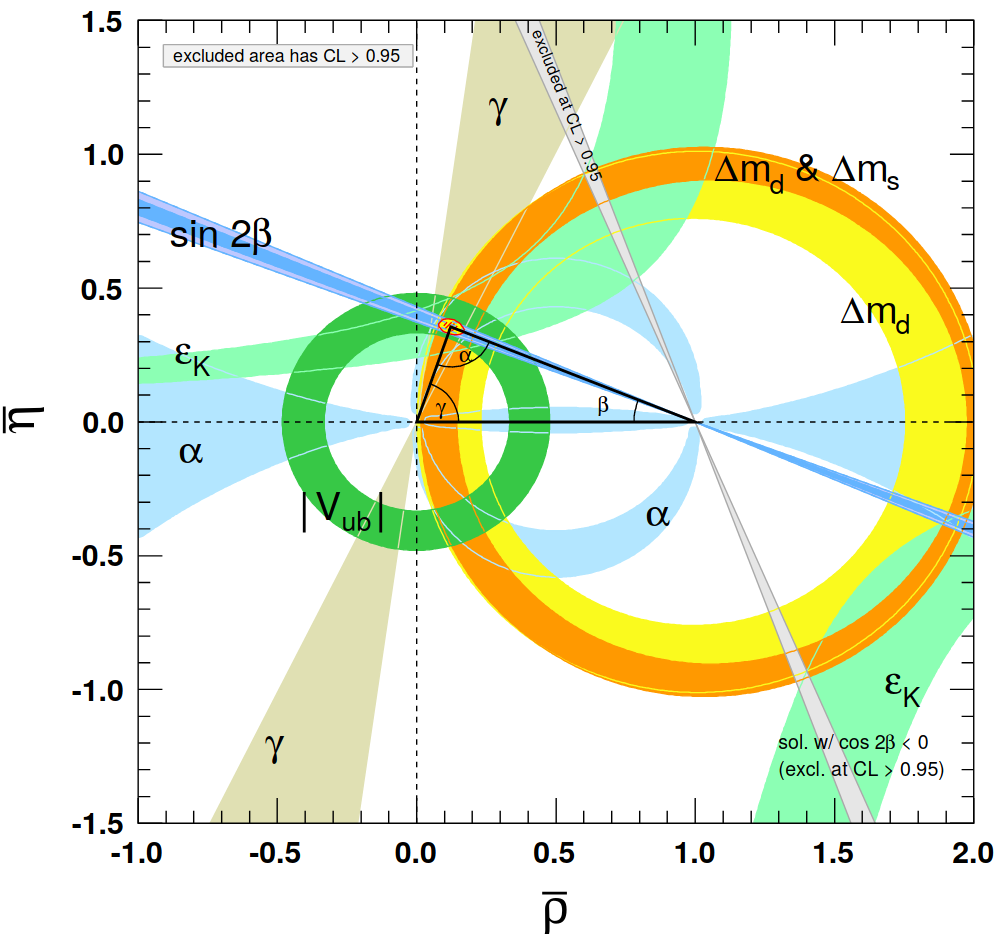
\includegraphics[width=0.55\textwidth]{figures/sm_theory/unitarity_triangle.png}
    \caption{\label{fig:unitarity_triangle}The constraints on the unitarity triangle in the $\bar{\rho},\bar{\eta}$ plane.
    Shaded areas represent  95\% confidence limits from different measurements constraining various angles of the triangle.
    Credit to Ref.~\cite{Workman:2022ynf}.
    }
\end{figure}

\section{The case for \texorpdfstring{$B$}{B} physics}\label{sec:bphysics_case}

The $B$ meson is the lightest hadron that contains a $b$ quark.
The decay of the unstable $b$ quark always contains a flavour-changing process via weak interaction.
Therefore, the study of their decays opens the possibility of measuring a wide range of parameters of the \SM, including the \CKM matrix, $\mathcal{CP}$ violation measurements, lepton mass measurements etc.
Furthermore, significant inconsistencies from the theoretical expectations may lead to breakthroughs in the theoretical understanding of Nature.
Some of the questions that are pursued through the study of $B$ mesons ($B$ physics) are \cite{Belle-II:2018jsg}:
\begin{itemize}
    \item What are additional sources of $\mathcal{CP}$ violation?
    \item Can there be additional Higgs bosons in Nature?
    \item How does dark matter fit in the Standard Model?
    \item Can the left-right symmetry of Nature, broken in weak interactions, be restored?
    \item Can charged lepton flavour-changing processes exist in Nature?
\end{itemize}

To exploit the properties of $B$ meson decays, a special type of experiments, known as \textit{$B$ factories}, are designed to study $B$ mesons.
They will be introduced in \Cref{ch:belle2}.

\section{The decay rate of \texorpdfstring{\BtoXsdgamma}{B->Xsg}}\label{sec:btosgamma_totalrate_theory}

In the \SM, $b\ra s$ transitions are mediated by so-called flavour-changing neutral currents.
These processes cannot occur directly and only happen through loops mediated by virtual particles.
One of the decay channels used to study these transitions is the so-called rare radiative $b\ra s\g$ and $b\ra d\g$ decays.
Due to the confinement effect and the hadronisation of the quarks, in reality, they manifest as \BtoXsgamma or \BtoXdgamma, where $X_s$ and $X_d$ denote any meson state originating from the $s$ or $d$ quark hadronisation.
The leading \SM diagrams for \BtoXsdgamma (used to collectively identify $X_s$ and $X_d$ states) processes are shown in \Cref{fig:sm_diagrams}.

\begin{figure}[htbp!]
\resizebox{0.66\textwidth}{!}{
    \subcaptionbox{\label{fig:sm_diagrams}}{
        \begin{tikzpicture}
\begin{feynman}
\vertex (i1){b};
\vertex[right =1.2cm of i1] (a) ;
\vertex[right=0.85cm of a] (b);
\vertex[right=0.85cm of b] (c);
\vertex[right=1.2cm of c] (o1) {s,d};
\vertex[below=2em of c] (g1);
\vertex[right=2em of g1] (o2) {$\gamma$};

\diagram* {
(i1) -- [fermion] (a) -- [boson, edge label =\(W^{\pm}\)] (c) -- [fermion] (o1),
(a) -- [fermion,half left, edge label = \(uct\)] (c),
(b) -- [photon] (o2),
};
\end{feynman}
\end{tikzpicture}

        \begin{tikzpicture}
\begin{feynman}
\vertex (i1){b};
\vertex[right =1.2cm of i1] (a);
\vertex[right=0.85cm of a] (b);
\vertex[right=0.85cm of b] (c);
\vertex[right=1.2cm of c] (o1) {s,d};
\vertex[below=2em of c] (g1);
\vertex[right=2em of g1] (o2) {$\gamma$};

\diagram* {
(i1) -- [fermion] (a) -- [fermion, edge label =\(uct\)] (c) -- [fermion] (o1),
(a) -- [boson,half left, edge label = \(W^{\pm}\)] (c),
(b) -- [photon] (o2),
};
\end{feynman}
\end{tikzpicture}



    }
}
\resizebox{0.33\textwidth}{!}{
\subcaptionbox{\label{fig:bsm_diagrams}}{
    \begin{tikzpicture}
\begin{feynman}
\vertex (i1){b};
\vertex[right =1.2cm of i1] (a) ;
\vertex[right=0.85cm of a] (b);
\vertex[right=0.85cm of b] (c);
\vertex[right=1.2cm of c] (o1) {s,d};
\vertex[below=2em of c] (g1);
\vertex[right=2em of g1] (o2) {$\gamma$};

\diagram* {
(i1) -- [fermion] (a) -- [scalar, edge label =\(H^{\pm}\)] (c) -- [fermion] (o1),
(a) -- [fermion,half left, edge label = \(uct\)] (c),
(b) -- [photon] (o2),
};
\end{feynman}
\end{tikzpicture}

}
}
\caption{\label{fig:b_to_s_gamma_diagrams}
The Feynman diagrams for radiative $b\ra s(d)$ transitions. 
\Cref{fig:sm_diagrams} shows the leading-order \SM diagrams, where the $b\ra s(d)$ transition occurs via electroweak loops.
One possible beyond-\SM scenario where this transition is mediated by a charged Higgs boson particle is shown in \Cref{fig:bsm_diagrams}.
}
\end{figure}

Since \BtoXsdgamma decays proceed via $b\ra s(d)\g$ transitions, they are sensitive probes for beyond-Standard-Model (\BSM) particles. 
The leading contributions in the \SM only happen via one-loop diagrams, as seen in \Cref{fig:b_to_s_gamma_diagrams}.
The electroweak loop can get contributions from $u,c,t$ quarks but they are suppressed as followed by the Glashow-Iliopoulos-Maiani mechanism~\cite{Glashow:1970gm}.
Therefore, the loop is dominated by the much heavier top quark \cite{Mannel:2001vn}. 
The masses of possible \BSM weakly-interacting particles that can appear in the loops may be as high as \order{(100~\tev)} \cite{Misiak:2020vlo} which makes studying these decays appealing.

The decay rate of \BtoXsdgamma involves both weak and strong interactions.
The typical energy scale of these interactions is much lower than the electroweak scale: $\sim\order(m_W)$.
This motivates approximating the interactions mediated by heavy $Z$ and $\Wpm$ bosons by an effective point-like vertex.
An effective Lagrangian describing the $\b\to\s(d)\g$ can be written as~\cite{Kaminski:2012eb,Misiak:2015xwa}:
\begin{equation}\label{eq:effective_lagrangian}
    \mathcal{L}_{\mathrm{eff}} = \frac{4G_F}{\sqrt{2}}V_{tq}^*V_{tb}\left[\sum^{8}_{i=1}\mathcal{C}_i(\mu)\mathcal{O}_i(\mu)
                                                + \frac{V^*_{uq}V_{ub}}{V^*_{tq}V_{tb}}\sum^{2}_{i=1}\mathcal{C}_i(\mu)(\mathcal{O}_i(\mu)-\mathcal{O}_i^u(\mu))\right],
\end{equation}
where $G_F$ is the Fermi constant, $q\in\{s,d\}$, and $V_{ij}$ are the appropriate \CKM matrix elements.
The factors $\mathcal{C}_i$, known as \textit{Wilson coefficients}, encode the high-energy weak contributions and can be calculated perturbatively.
The operators $\mathcal{O}_i$ describe the effective point-like interactions vertices in the effective field theory.
The renormalisation scale, $\mu$, needs to be chosen close to the typical energies of the studied process.
For the calculations of the total decay rate of radiative $B$ meson decays it is conventionally set to be of the order of the $b$ quark mass: $\mu\sim m_b$.

The exact expressions of operators $\mathcal{O}_i$, relevant for \btosgamma transitions, are given in \Cref{sec:appendix_local_opperators}, while the sketches of effective processes that they represent are given in \Cref{fig:b_to_s_gamma_effective}.
\begin{figure}[htbp!]
    \begin{equation*}
    \mathcal{L}_{\mathrm{eff}} \propto
\mathcal{C}_7 \times
\Biggl[
\raisebox{5pt}{
\resizebox{0.085\textwidth}{!}{
\feynmandiagram [small, inline=(b.base), vertical=b to d] {
    a --  b [dot] -- c,
    b -- [boson] d [particle=$\gamma$],
    };
}
}\Biggr]
+
\mathcal{C}_8 \times
\Biggl[
\raisebox{5pt}{
\resizebox{0.085\textwidth}{!}{
\feynmandiagram [small, inline=(b.base), vertical=b to d] {
    a --  b [dot] --  c,
    b -- [boson] d [particle=$g$],
    };
}
}\Biggr]
+
\sum_i^{1,...,6}
\mathcal{C}_i\times
\Biggl[
\raisebox{3pt}{
\resizebox{0.085\textwidth}{!}{
\feynmandiagram [small, inline=(b.base), horizontal=a to c] {
    a --  b [dot] --  c,
    d --  b -- e,
    };
}
}\Biggr]
\end{equation*}
\caption{\label{fig:b_to_s_gamma_effective}
Schematic representation of the \SM effective $\mathcal{L}$ governing to \BtoXsgamma. 
The effective interactions are normalised by the Wilson coefficients, $C_i$, and described by operators $O_i$ (see \Cref{sec:appendix_local_opperators}) whose sketches are shown here.
They correspond to the effective Lagrangian in \Cref{eq:effective_lagrangian}.
}
\end{figure}
Coefficients $\mathcal{C}_{3-6}$ have been calculated and shown to be small, therefore the most important contributions arise from $\mathcal{O}_{1,2,7,8}$ \cite{Chetyrkin:1996vx,Misiak:2020vlo}.
Furthermore, the ratio $V^*_{uq}V_{ub}/V^*_{tq}V_{tb}$ is small for the case of $q=s$ \cite{Charles:2015gya}, and the terms including $\mathcal{O}^u_i$ are relevant only as higher-order corrections of the total decay rate~\cite{Misiak:2015xwa}.
The latter point does not hold for the $\b\to\d$ case, where the $V^*_{uq}V_{ub}/V^*_{tq}V_{tb}$ multiplied term is not numerically small and contributes already at the leading-order.
However, for the rest of this Section, $\b\to\s\g$ is the main focus unless explicitly stated otherwise.

The total decay rate of the inclusive \BtoXsgamma is modelled as the rate of the parton decay, 
taking advantage of the quark-hadron duality and \textit{local operator product expansion} \cite{Peskin:1995ev,Buchalla:1995vs,Buras:1998raa}.
In particular, additional non-perturbative components need to be considered for the \SM calculation of the total decay rate \cite{Misiak:2015xwa}:
\begin{equation}\label{eq:btosgammarate_nonp}
    \Gamma(B\ra\X_s\g) = \Gamma(b\ra s\g) + \delta\Gamma_{\mathrm{non-p.}},
\end{equation}
$\Gamma(b\ra s\g)$ is the perturbatively calculable rate of $b$ quarks decaying into charmless partons, 
and $\partial\Gamma_{non-p.}$ is the non-perturbative contribution arising outside of local operator product expansion when accounting for the fact that the $b$ quark is not stationary inside the bound $B$ meson state.
As long as an appropriately low photon energy threshold (in the decaying $B$ meson rest frame) is chosen, the non-perturbative effects in \Cref{eq:btosgammarate_nonp} can be considered smaller as they `average out' over the spectrum.
Due to contributions from $\ccbar$ resonances at low-\Egamma, the threshold is conventionally chosen at $\Egamma>1.6~\gev$ \cite{Misiak:2009nr}.
Until recently, a 5\% uncertainty was associated with this assumption \cite{Benzke:2010js}. 
However, recent developments in understanding the non-perturbative effects \cite{Gunawardana:2019gep} led to an improved treatment of these uncertainties \cite{Misiak:2020vlo}.
One notable example of non-perturbative effects that are retained in total branching fraction calculations is the so-called resolved photon contributions.
These contributions are a result of the photon coupling directly to partons instead of the effective weak interaction vertex.
The origin of the non-perturbative contribution will be further discussed with the differential decay rate in \Cref{sec:btosgamma_spectrum_theory}.
It will also be seen that the threshold for \Egamma is motivated also from the experimental side, as a large background process contamination is present in the low-\Egamma region.

Using operator product expansion, one can calculate the matrix element $|\mel*{s\g}{\mathcal{L}_{\mathrm{eff}}}{b}|^2$ and integrate it from a chosen energy threshold, $\Egamma>E_0$. 
Then the perturbative decay rate can be written as \cite{Misiak:2020vlo}:
\begin{equation}\label{eq:theory_decay_rate}
    \Gamma(b\ra\s\g) = \frac{G^2_F m_{\mathrm{b}}^5 \alpha_{\mathrm{em}}}{32\pi^4}|V_{ts}^*V_{tb}|^2\sum_{i,j=1}^8\mathcal{C}^{\mathrm{eff}}_{i}(\mu_b)\mathcal{C}^{\mathrm{eff}}_{j}(\mu_b)\hat{G}_{ij}(E_0,\mu_b),
\end{equation}
where $m_{\mathrm{b}}$ is the $b$ quark pole mass, and $\alpha_{\mathrm{em}}$ is the fine-structure constant.
The $C_{i}^{\mathrm{eff}}(\mu_b)$ coefficients represent effective Wilson coefficients \cite{Buras:1993xp} that are independent of the renormalisation scheme and defined through linear combinations of the Wilson coefficients of \Cref{eq:effective_lagrangian}.
Finally, the functions $\hat{G}_{ij}$ encapsulate the terms describing the interference between the operators $\mathcal{O}_{i,j}$, which arise in the squared matrix element.
As already mentioned before, the dominant terms arise from a handful of operators $\mathcal{O}_i$, and the combined efforts to calculate them have brought \BtoXsgamma theoretical estimates to the next-to-next-to-leading-order precision.
The dominant functions $\hat{G}_{77}$ \cite{Asatrian:2006rq}, $\hat{G}_{78}$ \cite{Asatrian:2010rq}, and $\hat{G}_{(1,2)7}$ \cite{Boughezal:2007ny,Misiak:2020vlo} have been evaluated.
Contributions from $\hat{G}_{(1,2,8)8}$ \cite{Ferroglia:2010xe,Misiak:2010tk} have also been calculated.
As the calculations have already reached next-to-next-to-leading-order precision, even contributions involving $\mathcal{O}_{i}^u$ are accounted for \cite{Huber:2014nna}.
The mixing of $\mathcal{O}_{1-6}\to\mathcal{O}_8$ has been also described \cite{Czakon:2006ss}. 
Some of the next-to-next-to-leading-order corrections depend on the mass of the charm quark.
However, as the evaluation of such corrections at the physical mass of the charm quark is complicated, the mass is interpolated between $m_c=0$ and $m_c\gg m_b$ \cite{Misiak:2019ccp}.

\Cref{eq:theory_decay_rate} contains a 5th power dependence on the ill-defined pole mass of the $b$~quark.
Furthermore, uncertainties arising from the CKM matrix element determination also directly enter the calculation.
To minimise the uncertainties related to these values, the calculation of \btosgamma decay rate is usually normalised to the semi-leptonic decay rate $b\rightarrow u\ell\nu$.
An alternative choice is the experimentally more attainable $b\rightarrow c\ell\bar{\nu}$, 
however, using the charmless decay rate allows separating the $m_c$ determination problem from the problem of calculating higher-order corrections.
In doing so, the decay rate ratio is expressed as \cite{Gambino:2001ew}:
\begin{equation}
    \frac{\Gamma(\b\to\s\g)_{\Egamma>E_0}}{|V_{cb}/V_{ub}|^2 \Gamma(\b\to\u \ell\nub)} = \left|\frac{V_{ts}^*V_{tb}}{V_{cb}}\right|^2 \frac{6\alpha_{\mathrm{em}}}{\pi}P(E_0).
\end{equation}
Here, $P(E_0)$ denotes the perturbatively calculable contribution. 
Replacing $b\ra B$, as seen with \Cref{eq:btosgammarate_nonp}, required the introduction of a non-perturbative correction, $N(E_0)$:

\begin{equation}\label{eq:normalised_br}
    \frac{\Gamma(\BtoXsgamma)_{\Egamma>E_0}}{\Gamma(\B\to X_c\ell\nu_\ell)} = \frac{\mathcal{B}(\BtoXsgamma)_{\Egamma>E_0}}{\mathcal{B}(\B\to X_c\ell\nu_\ell)} = \left|\frac{V_{ts}^*V_{tb}}{V_{cb}}\right|^2\frac{6\alpha_{\mathrm{em}}}{\pi C}[P(E_0)+N(E_0)].
\end{equation}
The additional semileptonic phase-space factor:
\begin{equation}
    C = \left|\frac{V_{ub}}{V_{cb}}\right|^2 \frac{\Gamma(\B\to X_c\ell\bar{\nu})}{\Gamma(\B\to X_u\ell\bar{\nu})},
\end{equation}  
accounts for the choice to use the $B\rightarrow X_c\ell\bar{\nu}$ as a normalisation channel for the total decay rate. 
It is determined using the experimental value of the branching ratio of $\B\to X_c \ell\bar{\nu}$, which is known to a high precision \cite{Alberti:2014yda,Workman:2022ynf}.
This choice is preferable compared to the \mbox{$|V_{ub}|$-suppressed} and more model-dependant $\B\to X_u\ell\bar{\nu}$.

At the leading-order, where non-perturbative effects are disregarded, effects from $\mathcal{C}_{2,7,8}$ are the most important and this can be expressed in a compact form \cite{Buras:1993xp}:
\begin{equation}\label{eq:total_decay_rate_leading_order}
    \frac{\mathcal{B}(\BtoXsgamma)}{\mathcal{B}(\B\to X_c\ell\nu_\ell)} = \left|\frac{V_{ts}^*V_{tb}}{V_{cb}}\right|^2\frac{6\alpha_{\mathrm{em}}}{\pi C}|\mathcal{C}_{7}^{(0)\mathrm{eff}}(\mu)|^2.
\end{equation}
Here $\mathcal{C}_{7}^{(0)\mathrm{eff}}(\mu)$ is the effective leading-order Wilson coefficient which was briefly introduced before.
At leading-order, it takes the form:
\begin{equation}\label{eq:effective_c7}
    \mathcal{C}_{7}^{(0)\mathrm{eff}}(\mu) = \eta^{16/23}\mathcal{C}^{(0)}_7(\mu) + \frac{8}{3} \left(\eta^{14/23}-\eta^{16/23}\right)\mathcal{C}^{(0)}_8(\mu) + \mathcal{C}^{(0)}_2(\mu) \sum_i^8h_i\eta^{a_i},
\end{equation}
where the \SM coefficients $\mathcal{C}_{2,7,8}^{(0)}$ are expressed in terms of the ratio of $\Wpm$ and top-quark masses, $x=(m_t/m_W)^2$:
\begin{align}\label{eq:leading_order_wilson_coeffs}
    \begin{split}
        \mathcal{C}_2^{(0)}(\mu) &= 1;\\
        \mathcal{C}_7^{(0)}(\mu) &= F_7^{(1)}(x) \equiv \frac{3x^3-2x^2}{4(x-1)^4}\ln x + \frac{-8x^3-5x^2+7x}{24(x-1)^3};\\
        \mathcal{C}_8^{(0)}(\mu) &= F_8^{(1)}(x) \equiv \frac{-3x^2}{4(x-1)^4}\ln x + \frac{-x^3+5x^2+2x}{8(x-1)^3}.\\
    \end{split}
\end{align}
The coefficient $\eta$ is expressed as $\eta=\alpha_s(m_W)/\alpha_s(\mu)$, whereas $h_i$ and $a_i$ are the eigenvalues of a scheme-independent matrix $\gamma^{(0)\mathrm{eff}}$, 
which is defined in Appendix A of Ref.~\cite{Buras:1993xp}.
The matrix $\gamma^{(0)\mathrm{eff}}$ governs the leading-order strong interaction corrections to $\b\ra\s\g$, and its elements appear in the renormalisation group equation of the effective Wilson coefficients.

Considering the effective interactions in \Cref{fig:b_to_s_gamma_effective}, it may seem peculiar that $\mathcal{O}_{2,8}$ are important at the leading-order.
However, because \BtoXsgamma receives Glashow-Iliopoulos-Maiani suppression terms $(\sim m_q^2/m_W^2)$, two-loop contributions involving a gluon exchange $(\sim\ln m_t^2/m_b^2)$ are important \cite{Bertolini:1986th}.
In the absence of \QCD, one has $\eta=1$ and \BtoXsgamma decays are governed solely by the photonic dipole exchange.
Consider evaluating \Cref{eq:effective_c7} explicitly for $m_t=170~\gevcc$, $\mu=5~\gevcc$, $\alpha_s(m_Z)=0.118$~\cite{Buras:1998raa}:
\begin{align}
    \begin{split}
        \mathcal{C}_7^{(0)\mathrm{eff}}(\mu_b) &\approx 0.695 \cdot \mathcal{C}_7^{(0)}(\mu) + 0.085 \cdot \mathcal{C}_8^{(0)}(\mu) - 0.158 \cdot \mathcal{C}_2^{(0)}(\mu)  \\ 
                          &\approx 0.695 \cdot (-0.193) + 0.085 \cdot (-0.096) - 0.158\\
                          &\approx -0.300. \\
    \end{split}
\end{align}
The additive \QCD two-loop contributions including terms with $\mathcal{C}_8$ and $\mathcal{C}_2$ enhance the decay rate significantly.
On the other hand, multiplicative \QCD correction in the first term suppresses the decay rate.

Beyond the leading-order approximation, one has to take into account the full form of \Cref{eq:normalised_br}.
A sketch of the next-to-leading-order can be found in Ref.~\cite{Gambino:2001ew}, whereas the most up-to-date total decay rate calculation is described in Ref.~\cite{Misiak:2020vlo}, and references therein.
A detailed description of the higher-order calculation of the total \BtoXsgamma decay rate is beyond the scope of this thesis, but such calculations can be followed up in the references introduced in this Chapter, such as Ref.~\cite{Misiak:2020vlo} that includes the most up-to-date estimation of the total decay rate of \BtoXsgamma in the \SM:
\begin{equation}\label{eq:btosgamma_theoretical}
    \mathcal{B}(\BtoXsgamma) = (3.40\pm 0.17) \times 10^{-4}.
\end{equation}
\sloppy For $\BtoXdgamma$, as evident from \Cref{eq:effective_lagrangian}, 
the result is suppressed by a factor \mbox{$|V_{td}/V_{ts}|^2\approx4.2\%$} with respect to the \BtoXsgamma result.
Evaluating the decay with the exchanged CKM factors and other previously discussed caveats~\cite{Misiak:2015xwa}:
\begin{equation}\label{eq:btodgamma_theoretical}
    \mathcal{B}(\BtoXdgamma) = (0.173\pm^{0.12}_{0.22}) \times 10^{-4}.
\end{equation}

For \BtoXsgamma, the uncertainties in \Cref{eq:btosgamma_theoretical} arise from unevaluated higher-order effects, the necessity to perform an interpolation in $m_c$, and a parametric uncertainty that also encodes the non-perturbative effects.
The first two amount to $3\%$ each, whereas the last is considered at $2.5\%$. 
This amounts to a total uncertainty of approximately $5\%$.
For significant accuracy improvements in the future, higher-order calculations will not be sufficient.
It is necessary to remove the dependence on $m_c$ interpolation and improve the treatment of the parametric uncertainties (non-perturbative effects) to go below the $\sqrt{3^2+2.5^2}\approx3.9\%$ uncertainty.

\section{The photon energy spectrum of \texorpdfstring{\BtoXsdgamma}{B->Xsg}}\label{sec:btosgamma_spectrum_theory}

It was already briefly discussed (when introducing \Cref{eq:btosgammarate_nonp}) that theoretical and experimental evaluations of the total \BtoXsgamma decay rate employ a photon energy threshold.
The non-perturbative effects that occur at different energy scales compared to the effective $b\ra\s\g$ transition can be partially integrated out in a treatment of the total decay rate.
However, the choice of a lower threshold spoils this approximation and introduces non-perturbative corrections.
These effects directly manifest as differences in the shape of the photon energy spectrum.

At the leading-order, $b\ra\s(\d) \g$ is a two-body decay, which means that the differential decay rate peaks near the half of $b$ quark mass, $m_b/2\sim E_{\g}$.
It is also clear that photon energies larger than half of the $B$ meson mass, $E_{\g}>m_B/2$ are not allowed.
Higher-order effects, such as gluonstrahlung and the Fermi motion of the $b$ quark within the $B$ meson, smear the distribution.
The necessity to account for all of these effects occurring at different energy scales motivates the use of soft-collinear effective theory to describe the \BtoXsgamma photon energy spectrum \cite{Neubert:2004qw,Ligeti:2008ac}.
It allows factorising different contributions to the decay rate, $d\Gamma$, into terms originating from effective hard-interaction vertices, collinear particles and soft particles:
\begin{equation}\label{eq:differential_decay_rate_SCET}
    d\Gamma \propto \mathcal{H} \times \mathcal{J} \otimes \mathcal{S}.
\end{equation}
$\mathcal{H}$, $\mathcal{J}$, $\mathcal{S}$ represent the hard, jet and hadronic-soft functions, respectively, with $\otimes$ symbolising convolution between the two terms.
It is further assumed that the $\mathcal{S}$ can be factorised into a partonic soft function, $\mathcal{S}_{\mathrm{partonic}}$, and a non-perturbative \textit{shape function}, $\mathcal{F}$:

\begin{equation}\label{eq:factorisation}
    \mathcal{S} = \mathcal{S}_{\mathrm{partonic}} \otimes \mathcal{F},
\end{equation}
which means that the application of soft-collinear effective theory is fully capable to separate perturbative and non-perturbative contributions in the differential decay rate of \BtoXsgamma.
This is shown graphically in \Cref{fig:xsgamma_theory_sketches}, which sketches out the leading-order perturbative and non-perturbative effects in describing the \BtoXsgamma spectrum.

Due to the larger \BtoXsgamma decay rate and an overall smaller background process rate, experimental values have the highest precision around the peak region.
However, from the theory side, the peak part is mostly governed by non-perturbative effects, encoded within the shape function \cite{Ligeti:2008ac}.
The shape function encodes the $b$ quark residual momentum distribution within the $B$ meson. 
Therefore, a reliable theoretical description of the shape function is critical to make sensible experimental and theoretical comparisons of the photon energy spectrum. 

\begin{figure}[htbp!]
    \centering
    \subcaptionbox{\label{fig:theory_to_experiment}}{
        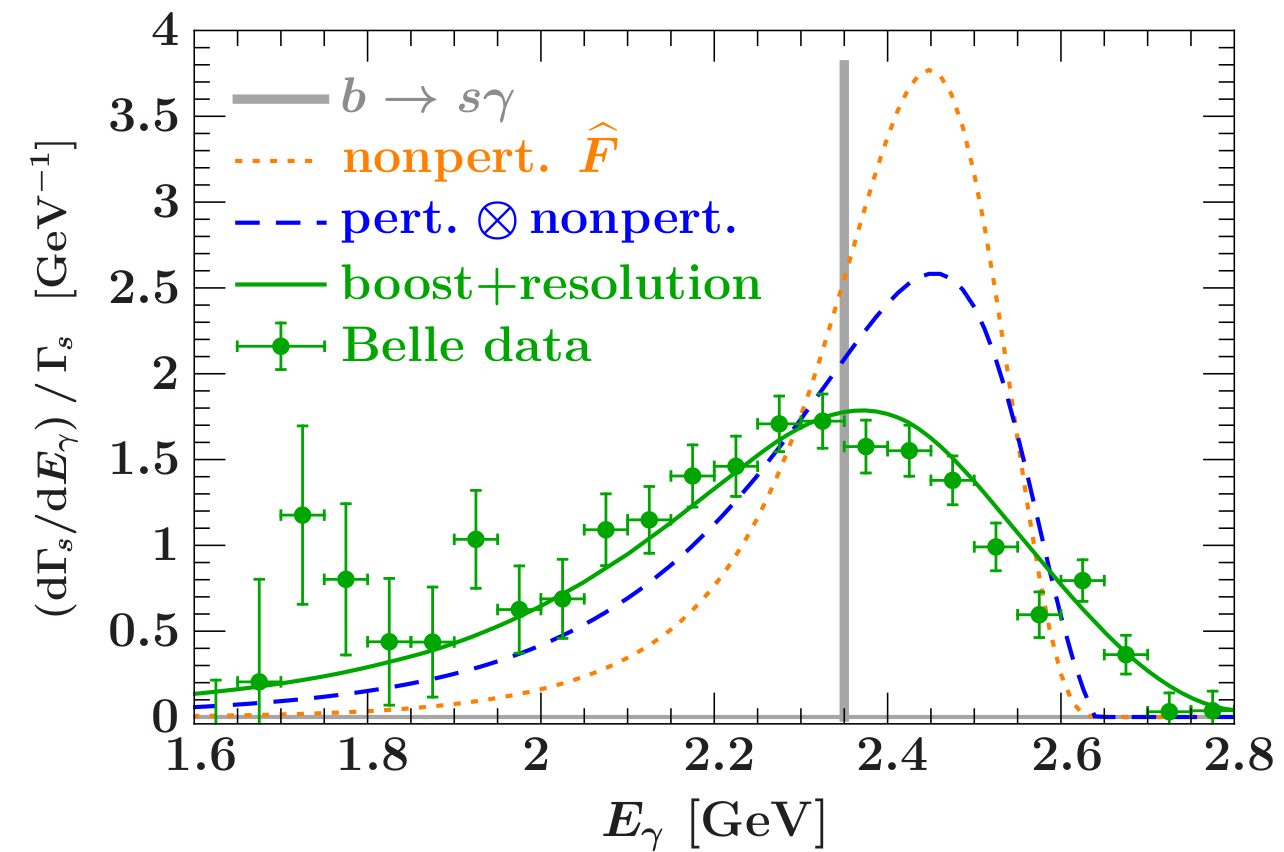
\includegraphics[width=0.45\textwidth]{figures/theory/xsgamma_theory_to_experiment.png}
    }
    \subcaptionbox{\label{fig:theory_ingredients_schematic}}{
        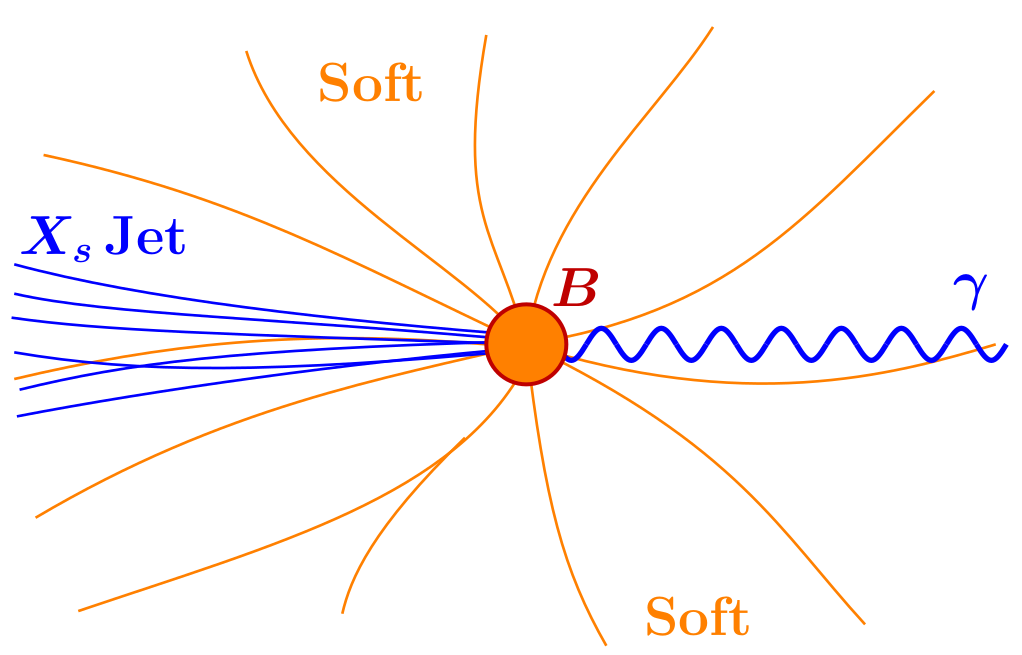
\includegraphics[width=0.45\textwidth]{figures/theory/xsgamma_theory_components.png}
    }
    \caption{\label{fig:xsgamma_theory_sketches} 
    The schematic representation of the theoretical \BtoXsgamma spectrum components and the comparison of them in data.
    Note that the figures are presented only for illustration purposes and do not represent a highly-accurate depiction.
    \Cref{fig:theory_to_experiment} represents the leading-order $\delta$ function spectrum, the non-perturbative shape function effects, and the convolution of these effects with the perturbatively calculable ones.
    It also includes the experimental effects, such as finite detector resolution.
    \Cref{fig:theory_ingredients_schematic} illustrates the origin of perturbative and non-perturbative effects in a \BtoXsgamma decay.
    Credit to Dr. Frank Tackmann for the Figures. 
    The data points in \Cref{fig:theory_to_experiment} correspond to the Belle measurement in \cite{Belle:2009nth}.}
\end{figure}

An additional motivation to study the shape function is the fact that it is a universal property of the $B$ meson at the leading-order in $1/m_b$ \cite{Neubert:1993um,Bigi:1993ex}.
This allows extracting the functional form by a precise experimental determination of the \BtoXsgamma spectrum and using it to improve the precision of other measurements.
For example, the measurement of $|V_{ub}|$ uses $B\rightarrow X_u \ell \bar{\nu}_{\ell}$ decays, however, it suffers orders-of-magnitude larger backgrounds due to the presence of $B\rightarrow X_c \ell \bar{\nu_{\ell}}$ in most phase-space regions.
In the regions where the $b\to c$ is kinematically-forbidden, the theoretical predictions for $B\rightarrow X_u \ell \bar{\nu_{\ell}}$ are dependent on the non-perturbative shape functions.
The extracted precise inputs from \BtoXsgamma could then be used to predict the $B\rightarrow X_u \ell \bar{\nu_{\ell}}$ spectra.
This is an important relationship which could lead to a model-independent evaluation of the $|V_{ub}|$ element \cite{Neubert:1993um}.

Let's consider \Cref{eq:differential_decay_rate_SCET,eq:factorisation} in a bit more detail.
Following the treatment of Ref.~\cite{Ligeti:2008ac}, the differential decay rate takes the form:

\begin{equation}\label{eq:differential_decay_simba}
    \frac{d\Gamma}{dE_{\gamma}} = 2\frac{G_F^2\alpha_{\mathrm{em}} m_b^5}{32\pi^4}|V_{ts}V_{tb}^*|^2 \mathcal{H}(x, \mu) \times \int dk \mathcal{P}(m_b, x - k, \mu_i) \mathcal{F}(k) + \order\left(\frac{\Lambda_{\mathrm{QCD}}}{m_b}\right),
\end{equation}
where $x=m_B-2\Egamma$, $\mathcal{P}$ is used to denote the perturbatively calculable $\mathcal{J}\otimes\mathcal{S_{\mathrm{partonic}}}$ and the symbolic convolution has now been replaced by an integration over a dummy momentum $k$.
The higher-order corrections introduce additional shape functions but are suppressed by a factor of $1/m_b$ \cite{Neubert:2002yx}.
Generally, $\mathcal{H}$ and $\mathcal{P}$ are calculable in perturbation theory (see Appendix A of \cite{Ligeti:2008ac}).
$\mathcal{H}$ is approximately expressed in terms of the effective Wilson coefficient $\mathcal{C}_7^{\mathrm{eff}}$. 
Moreover, at the leading-order in perturbation theory, $\mathcal{P}$ is expressed as a Dirac delta distribution:

\begin{equation}
    \mathcal{P}(m_b,k,\mu) = \delta(k) + \mathcal{O}(\alpha_s),
\end{equation}
and therefore integrating out the momentum $k$:
\begin{equation}\label{eq:integrated_egamma}
    \frac{d\Gamma}{d\Egamma} \propto |\mathcal{C}_7^{\mathrm{eff}}|^2 \mathcal{F}(x).
\end{equation}
This shows, as stated before, that the peak region (close to $m_b/2$) is governed by the shape function.
In this case, $|\mathcal{C}_7^{\mathrm{eff}}|$ is the normalisation of the spectrum.
The shape function can be formally expanded in its moments as \cite{PhysRevD.50.2037,Ligeti:2008ac}:
\begin{equation}\label{eq:shape_function_expansion}
    \mathcal{F}(x) = \sum_n \frac{(-1)^n}{n!} A_n \dv[n]{\delta(x)}{x},
\end{equation}
where 
\begin{equation}\label{eq:moments_of_shape_function}
    A_n = \int dk k^n \mathcal{F}(k).
\end{equation}
\Cref{eq:moments_of_shape_function} is the expression for the $n$-th moment of the shape function, where 
$A_0=1$ is fixed because the shape function is chosen to be normalised.
Note that if one naively neglects $n>1$ terms, the integral over the total $\Egamma$ of \Cref{eq:integrated_egamma} would take the form $\Gamma\sim|\mathcal{C}_7^{\mathrm{eff}}|^2$, which is consistent with \Cref{eq:total_decay_rate_leading_order}.
Therefore, for total decay rate calculations (such as the ones sketched in \Cref{sec:btosgamma_totalrate_theory}) it is enough to know the first moments of the shape function, as the more delicate $\mathcal{F}(k)$ dependence is suppressed at leading-orders.

For example, consider taking only terms up to the first order.
In such case, using the definition of an average,
\begin{equation}
    \expval{\Egamma} = \frac{\int d\Egamma \Egamma \dv{\Gamma}{\Egamma}}{\int d\Egamma \dv{\Gamma}{\Egamma}},
\end{equation}
the shape function is directly related to the average of the photon energy spectrum.
Similarly, the variance (and higher-order moments) contribute if more terms from \Cref{eq:shape_function_expansion} are considered.
As shown in Refs.~\cite{Bauer:1997fe,Kapustin:1995fk} (and others) two important relations emerge:
\begin{equation}
    \expval{\Egamma} \sim m_b/2+\order(\Lambda_{\mathrm{QCD}}); \quad \expval{\Egamma^2}-\expval{\Egamma}^2 \sim \lambda_1/3+\order(\Lambda_{\mathrm{QCD}}),
\end{equation}
with the $b$ quark pole mass, $m_b$, the $b$ quark kinetic energy parameter, $\lambda_1$, and $\Lambda_{\mathrm{QCD}}$ is the chosen strong interaction energy scale.

The form of the shape function is not well-known and is non-perturbative, unlike the Wilson coefficients.
Therefore, theoretical and experimental comparisons always lead to modelling-related uncertainties.
There are many works which propose different ways to describe it \cite{Benson:2004sg,Lange:2005yw,Andersen:2005mj,Gambino:2007rp,Aglietti:2007ik,Bernlochner:2020jlt}.
For example, Ref.~\cite{Andersen:2005mj} describes it based on a technique called dressed gluon exponentiation.
The result of Ref.~\cite{Lange:2005yw} provides several functional forms of the shape function, based on the leading-order shape function that can be extracted from \BtoXsgamma decays.
An analysis by the SIMBA collaboration \cite{Bernlochner:2020jlt} describes a model-independent treatment of the shape function based on \Cref{eq:differential_decay_simba}.
In particular, any chosen shape function is expanded in a complete set of orthonormal basis functions, and can therefore be extracted, together with the normalisation, from a global fit to the available experimental results.
The strength of this approach is a consistent method to combine several experimental inputs for the extraction of the shape function and its moments.

One of the most commonly chosen inclusive \BtoXsgamma models for experimental analyses is known as the Kagan-Neubert model \cite{Kagan:1998ym}.
It provides a next-to-leading-order description of the inclusive \BtoXsgamma spectrum. 
In this model, the shape function takes a simple form:
\begin{equation}
    \mathcal{F}(x) = N\left(1-\frac{x}{m_B-m_b}\right)^a\exp{(1+a)\frac{x}{m_B-m_b}},
\end{equation}
The shape function satisfies the necessary moment constraints through these relations: $A_0=1,A_1 = 0,A_2=-\lambda_1/3$.
The parameter $a$ is also related to $A_2=(m_B-m_b)/(1+a)$.
Therefore, the shape function can be fully described by two free parameters $m_b$ and $\lambda_1$.
This functional expression is easy to implement and interpret.
Furthermore, the Kagan-Neubert model is readily available in the \texttt{EvtGen} Monte Carlo generator, commonly used by $B$ factories \cite{Ryd:2005zz}.
The \BtoXsgamma inclusive decay is implemented as the \texttt{BTOXSGAMMA} model within the generator. 
These points made it the conventional choice for an experimental description of the inclusive \Egamma spectrum in many past measurements.
The spectra, generated with varied values of $\lambda_1$ and $m_b$, using the kinetic scheme, are shown in \Cref{fig:knmodel_variation}, otherwise using the default \texttt{BTOXSGAMMA} setup.
\begin{figure}[htbp!]
    \subcaptionbox{\label{fig:knmodel_mb_variation}}{
        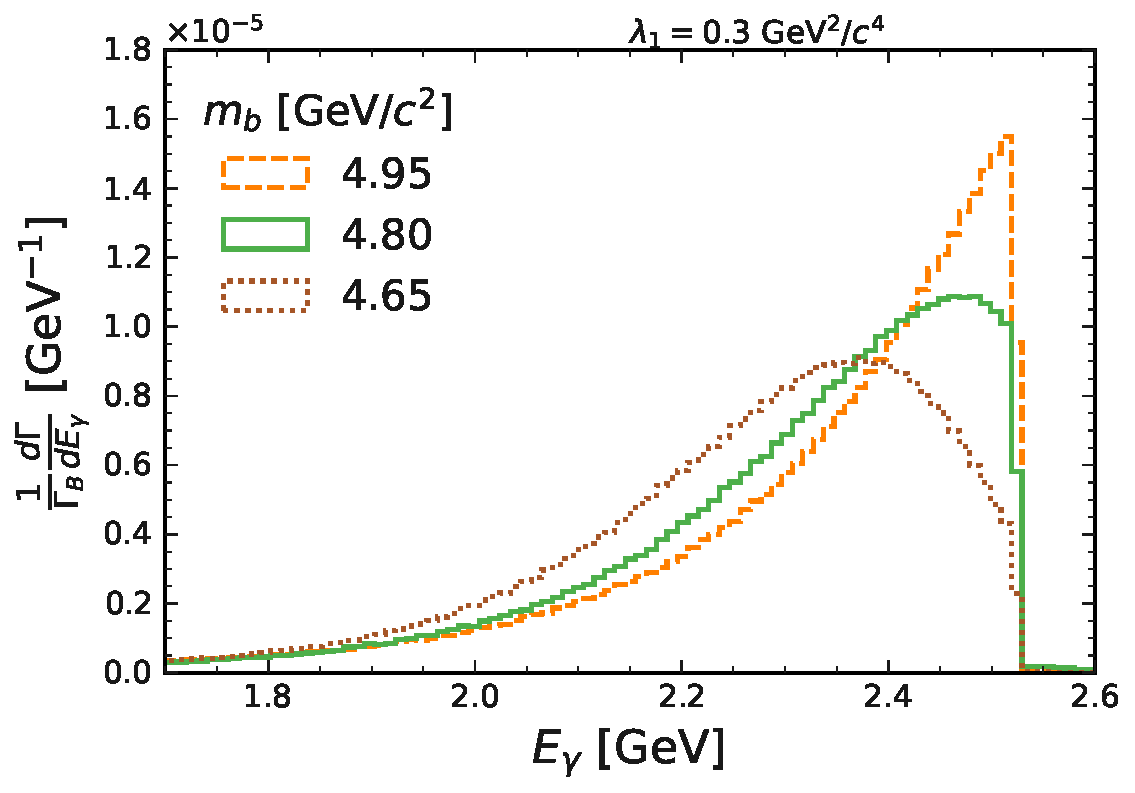
\includegraphics[width=0.45\textwidth]{figures/theory/xsgamma_spectrum_mb_variation.pdf}
    }
    \subcaptionbox{\label{fig:knmodel_lambda_variation}}{
        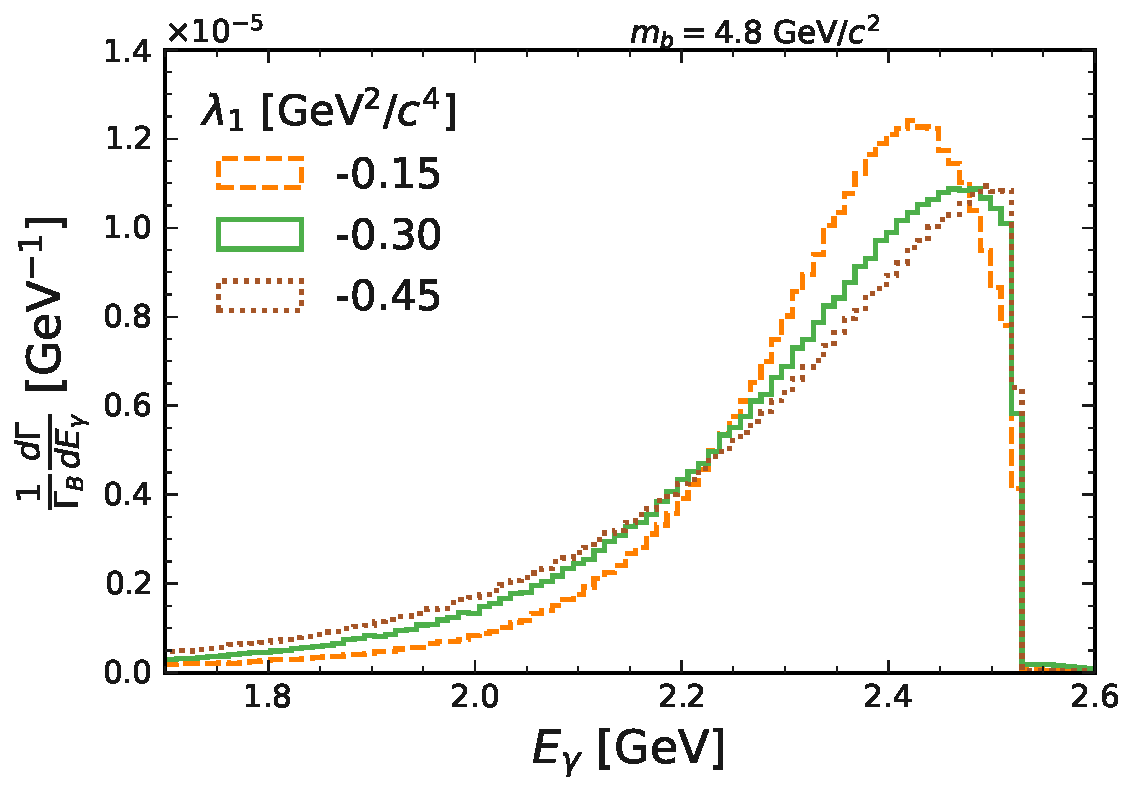
\includegraphics[width=0.45\textwidth]{figures/theory/xsgamma_spectrum_lambda_variation.pdf}
    }
    \caption{\label{fig:knmodel_variation}
    The \BtoXsgamma spectrum predicted by the Kagan-Neubert model, generated using the \texttt{EvtGen} generator's \texttt{BTOXSGAMMA} model.
    \Cref{fig:knmodel_mb_variation} shows how variations of $m_b$ affect the spectrum while keeping $\lambda_1$ constant.
    \Cref{fig:knmodel_lambda_variation} depicts the inverse scenario.
    The values here are provided in the kinetic scheme and correspond to those used by the authors of Ref.~\cite{Kagan:1998ym}.
    The generated spectra correspond to $10^6$ events of both $B^+$ and $B^0$ decay modes.
    The full line corresponda to the default setup used by \texttt{BTOXSGAMMA}.
    The model generates the $\Egamma$ spectrum for $m_{X_s}>1.1~\gevcc$, which corresponds to $\Egamma\lessapprox2.52~\gev$ (see \Cref{eq:mx_egamma_relation}).}
\end{figure}

The previous argument may also be used inversely: an accurate experimental measurement of the \BtoXsgamma spectrum
can be used to precisely determine the parameters $m_b$, $\lambda_1$ and higher moments of the shape function.
One such example is the aforementioned SIMBA collaboration result \cite{Bernlochner:2020jlt}.
The evaluated values of $m_b$ and $\lambda_1$ by the SIMBA collaboration from fitting available \BtoXsgamma experimental results are:

\begin{equation}\label{eq:simba_result}
    m_b^{1S} =4.750 \pm 0.043~\gevcc;  \quad \lambda^{\mathrm{inv}}_1 = -0.210\pm0.083~\gev^2/c^4, 
\end{equation}
where fitting, theoretical and parametric uncertainties are combined.
These results originate directly from experimental data fits and have slightly larger than world average uncertainties.
The superscripts $1S$ and `$\mathrm{inv}$' indicate a renormalisation scheme that is chosen by the authors.

The works presented in this thesis will use the Kagan-Neubert model to generate the inclusive photon energy spectrum.
The $m_b$ and $\lambda_1$ values measured by the SIMBA collaboration will be used, as they are extracted from all available experimental evidence, and contain slightly larger uncertainties making it a conservative estimate.
Generally, these parameters are heavily dependent on the renormalisation scheme that is chosen.
The relations provided in \cite{Ligeti:2008ac} will be used to transform the `$1S$/$\mathrm{inv}$' scheme to the kinetic scheme at the precision of $\order(\alpha_s^2)$, which can be used in the Kagan-Neubert model.

Lastly, it is also important to stress that the Kagan-Neubert (or any inclusive) model cannot generate resonant structures that the $m_{X_s}$ exhibits.
As a two body decay, $m_{X_s}$ and $\Egamma$ are directly related:
\begin{equation}
    m_{X_s}^2 = m_B^2 - 2m_B\Egamma.
\end{equation}
Therefore, the theoretical inclusive photon energy spectrum must always be interpreted in the picture of quark-hadron duality.
In the low-\Egamma region non-resonant and resonant decays are effectively indistinguishable as there are numerous available kinematic states.
The inclusive model describes the spectrum as an average of all the states, and this is further enhanced by resolution effects in experimental data (see \Cref{sec:unfolding}).
In the high-\Egamma region, however, the spectrum is dominated by several resonances, most notably the well-separated $B\rightarrow\Kstar(892)\gamma$.
A study by the authors of the Kagan-Neubert model \cite{Kagan:1998ym} shows that the inclusive model for $m_{X_s}\gtrsim 1.1~\gevcc$ should be supplemented by the resonant decays.
This approach is followed when implementing a model for the analysis in \Cref{sec:signal_model}

\section{New-physics opportunities in \safeBtoXsgamma decays}\label{sec:btosgamma_bsm}

The last Section introduced that \BtoXsgamma is important to constrain the \SM parameters, 
such as $m_b$, through the description of the $B$ meson shape function and its moments.
However, one of the main motivations to study \BtoXsgamma decays is their sensitivity to \BSM models.
Considering the \SM diagrams in \Cref{fig:b_to_s_gamma_diagrams}, any non-\SM particles that couple to quarks and/or photons could contribute.

If light particles that couple to quarks would exist, they would generally be expected to have been observed by now.
Therefore, the new degrees of freedom introduced by \BSM models are expected to be heavy.
In effective field theory terms:
\begin{equation}\label{eq:corr_wilson}
    \mathcal{C}_i^{\mathrm{SM}} \ra \mathcal{C}_i^{\mathrm{SM}} + \delta\mathcal{C}_i^{\mathrm{\BSM}}.
\end{equation}
That is, \BSM physics can manifest by modifying any Wilson coefficient contributing to the \btosgamma Lagrangian (\Cref{eq:effective_lagrangian}).
New Wilson coefficients may also be introduced by certain theories.
Some of the models which could exhibit these effects for \BtoXsgamma include 
two-Higgs-doublet models (\TwoHDM) \cite{Borzumati:1998tg,Bobeth:1999ww,Hermann:2012fc}, 
minimal supersymmetric models with minimal flavour violation \cite{Bobeth:1999ww,Borzumati:2003rr,Degrassi:2006eh,Freitas:2007dp}
and left-right symmetric models \cite{Bobeth:1999ww}.
More exotic models include 
general minimal-supersymmetric theories \cite{Ciuchini:2007ha},
models with extra dimensions \cite{Buras:2003mk,Agashe:2004cp,Haisch:2007vb,Freitas:2008vh},
the littlest Higgs models \cite{Buras:2006wk,Blanke:2006sb},
and so-called 331 models \cite{Promberger:2008xg}.

One of the most compelling \SM extensions is the set of the \TwoHDM models.
A thorough overview of different types of \TwoHDM models is presented in Ref.~\cite{Branco:2011iw}.
The model is attractive because it can be incorporated into many theories that provide insight into the long-standing issues of the \SM.
In supersymmetric theories, a second Higgs doublet is required to give masses to both $u$- and $d$-type quarks.
Furthermore, having a second Higgs doublet could allow solving the strong $\mathcal{CP}$ problem.
Finally, it may also provide answers to the baryon asymmetry observed in the Universe.
An example of a charged Higgs boson, a prediction of (but not exclusively) \TwoHDM models, contributing to the \btosgamma transition is shown in \Cref{fig:bsm_diagrams}.

Two main types of \TwoHDM models contribute in the quark sector with vanishing tree-level flavour-changing neutral current contributions:
so-called type-I \TwoHDM, where all quarks can couple to only one of the Higgs doublets, or
type-II \TwoHDM, where $u$-type quarks couple to one doublet and $d$-type couple to another.
In the \SM, a Lagrangian for a charged Higgs boson interaction with quarks, following these requirements, is \cite{Hermann:2012fc}:
\begin{equation}
    \mathcal{L}_{H^+} = \frac{1}{\sqrt{\sqrt8G_F}} \sum_{i,j=1} \bar{u}_i (A_u m_{u_i}V_{ij}P_L - A_d m_{d_j}V_{ij}P_R)d_jH^+ + \mathrm{h.c}.
\end{equation}
Here, $A_q$ are couplings, related to either $u$- or $d$-type quarks, with masses $m_u$ and $m_d$.
The sum runs over quark flavours $i$ and $j$, and $V_{ij}$ is the appropriate element of the CKM matrix.
$P_L$ and $P_R$ are the chiral projection operators, and h.c. implies an additional hermitian conjugate term. 
In the type-I \TwoHDM, the couplings to different $u$- and $d$-type quarks are:
\begin{equation}\label{eq:type1_hdm_couplings}
A_u = A_d = \frac{1}{\tan\beta},
\end{equation}
whereas for type-II \TwoHDM:
\begin{equation}\label{eq:type2_hdm_couplings}
    A_u = - \frac{1}{A_d} = \frac{1}{\tan\beta}.
\end{equation}
These couplings are expressed in terms of $\tan\beta$, which is the ratio of Higgs vacuum expectation values of the two doublets in these theories.
At the leading-order, the interactions are fully described by $\tan\beta$ and the mass of the charged Higgs, $m_{H^+}$, but these receive corrections at higher-orders related to other parameters in \TwoHDM or super-symmetric theories \cite{Feng:1996xv}.

The decay rate calculation for the \TwoHDM model in the above-described cases proceeds similarly as described in \Cref{sec:btosgamma_totalrate_theory}. 
By modifying the effective Wilson coefficients based on \Cref{eq:corr_wilson} and calculating appropriate corrections \cite{Ciuchini:1997xe}:
\begin{equation}\label{eq:partial_wilson_2hdm}
    \partial C_i^{(0)\TwoHDM} = 
    \begin{cases}
        0, & i=1,...,6;\\
        \frac{A_u^2}{3}F_i^{(1)}(y) - A_uA_dF_i^{(2)}(y), & i=7,8;\\
    \end{cases}
\end{equation}
where $F_i^{(1)}(y)$ have already been defined in \Cref{eq:leading_order_wilson_coeffs}, and
\begin{align}
    \begin{split}
    F_7^{(2)}(y) &= \frac{3y^2-2y}{6(y-1)^3}\ln y + \frac{-5y^2+3y}{12(y-1)^2},\\
    F_8^{(2)}(y) &= \frac{-y}{2(y-1)^3}\ln y + \frac{-y^2+3y}{4(y-1^2)},\\
    \end{split}
\end{align}
with $y = m_t^2/m_{H^+}^2$.
Using \Cref{eq:type1_hdm_couplings}, in the case of type-I \TwoHDM, the charged Higgs contribution takes the form $A\cot^2\beta-B\cot^2\beta$ which interferes with the \SM value destructively.
On the other hand, type-II \TwoHDM (\Cref{eq:type1_hdm_couplings}) will take the form $A\cot^2\beta+B$ which is always constructive \cite{Misiak:2017bgg}.

Higher-order corrections for \TwoHDM are provided in Refs.~\cite{Ciuchini:1997xe,Hermann:2012fc} and have reached the next-to-next-to-leading-order precision.
Based on \Cref{eq:partial_wilson_2hdm} and higher-order corrections, one can quantify the effect such models would have on the \BtoXsgamma branching fraction.
The dependence of the \BtoXsgamma decay rate on $m_{H^+}$ is shown in \Cref{fig:xsgamma_br_2hdm} for two particular cases of $\tan\beta$ (see later \Cref{fig:2hdm_limits}).

\begin{figure}[htbp!]
    \centering
    \subcaptionbox{\label{fig:xsgamma_2hdm_type1}}{
        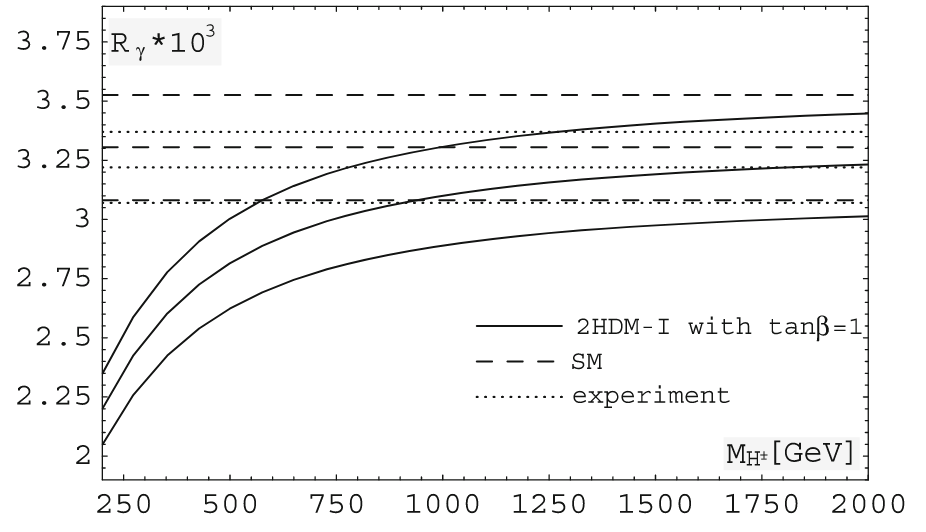
\includegraphics[width=0.48\textwidth]{figures/theory/xsgamma_2hdm_type1.png}
    }
    \subcaptionbox{\label{fig:xsgamma_2hdm_type2}}{
        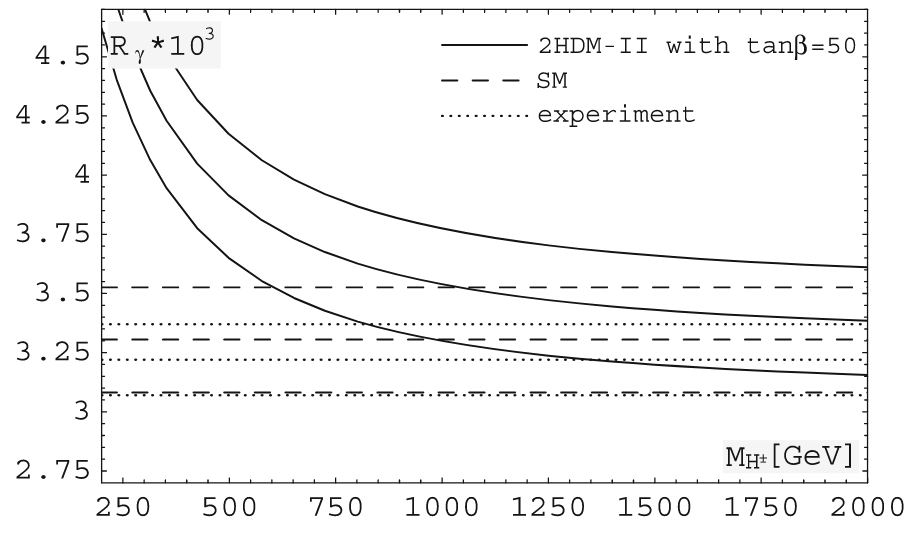
\includegraphics[width=0.48\textwidth]{figures/theory/xsgamma_2hdm_type2.png}
    }
    \caption{\label{fig:xsgamma_br_2hdm} 
    Variations of the \BtoXsgamma total decay rate (normalised by $B\rightarrow X_c \ell\bar{\nu}$ decay rate) as a function of the mass of the charged Higgs boson.
    \Cref{fig:xsgamma_2hdm_type1} shows the dependence for a type-I \TwoHDM model, whereas \Cref{fig:xsgamma_2hdm_type2} shows that for type-II \TwoHDM.
    The predictions are made assuming $\tan\beta=1$ and $\tan\beta=50$ for both types, respectively.
    The experimental bounds, as well as theoretical ones (not the most up-to-date), are shown as well.
    The Figures are taken from \cite{Misiak:2017bgg}.}
\end{figure}

The destructive (constructive) interference predicted by the type-I (type-II) \TwoHDM{s} is apparent in \Cref{fig:xsgamma_br_2hdm}.
Comparing the experimental and theoretical results seen in the figures allows $(\tan\beta,m_{H^+})$ parameter space ranges to be determined.
In both cases, as the charged Higgs mass increases, the predicted total decay rate approaches the \SM values.
This is because, in the $m_H^+\rightarrow\infty$ regime, the charged Higgs is effectively decoupled from the \SM.
The bounds imposed by next-to-next-to-leading-order \BtoXsgamma results on the $(m_{H^+},\tan\beta)$ space are shown in \Cref{fig:2hdm_limits}.

\begin{figure}[htbp!]
    \centering
        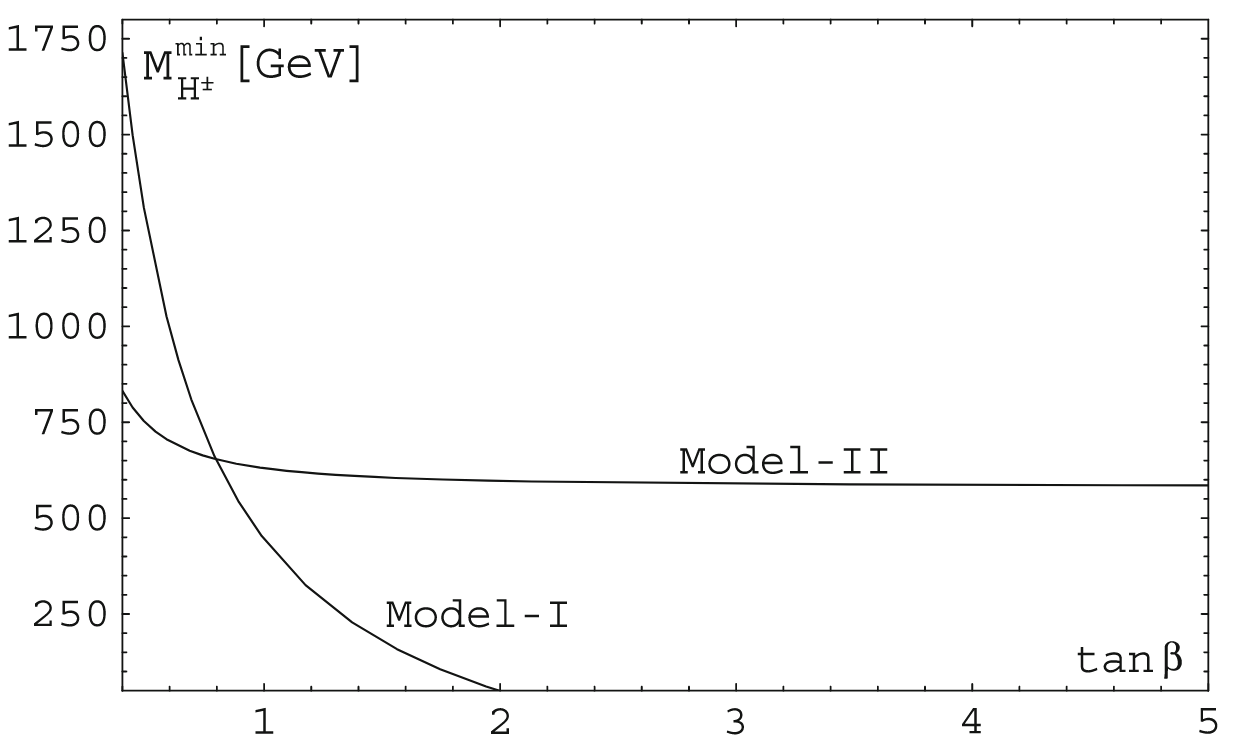
\includegraphics[width=0.5\textwidth]{figures/theory/xsgamma_2hdm_both_types.png}
    \caption{\label{fig:2hdm_limits} 
    Excluded (lower bound) for type-I and type-II \TwoHDM models in the $\tan\beta-m_{H^+}$ parameter space.
    The Figure begins at $\tan\beta>0.4$ as better alternative bounds exist below that range.
    The Figure is taken from \cite{Misiak:2017bgg}.}
\end{figure}

It can be seen that $(\tan\beta,m_{H^+})$ space is well-bounded for type-I and type-II \TwoHDM results.
The strongest bounds arise for type-I \TwoHDM results in the range of $\tan\beta\in(0.4,2)$.
On the other hand, type-II \TwoHDM saturates at the high $\tan\beta$ limit.
For values outside these ranges other experimental bounds are necessary \cite{Misiak:2017bgg}.
Using the methods laid out in this Section, Ref.~\cite{Misiak:2020vlo} rules out type-II \TwoHDM models with a charged Higgs lighter than $800~\gev$ at $2\sigma$.
A compatible result is also obtained in Ref.~\cite{Atkinson:2021eox}.